\documentclass[journal,12pt,onecolumn]{IEEEtran}
\usepackage{cite}
\usepackage{graphicx}
\usepackage{amsmath,amssymb,amsfonts,amsthm}
\usepackage{algorithmic}
\usepackage{graphicx}
\usepackage{textcomp}
\usepackage{xcolor}
\usepackage{txfonts}
\usepackage{listings}
\usepackage{enumitem}
\usepackage{listings}
\usepackage{pgf-pie}
\usepackage{mathtools,tfrupee}
\usepackage{gensymb}
\usepackage{comment}
\usepackage[breaklinks=true]{hyperref}
\usepackage{tkz-euclide} 
\usepackage{listings}
\usepackage{gvv}                                        
%\def\inputGnumericTable{}                                 
\usepackage[latin1]{inputenc} 
\usetikzlibrary{arrows.meta, positioning}
\usepackage{xparse}
\usepackage{color}                                            
\usepackage{array}                                            
\usepackage{longtable}                                       
\usepackage{calc}                                             
\usepackage{multirow}
\usepackage{multicol}
\usepackage{caption}
\usepackage{hhline}                                           
\usepackage{ifthen}                                           
\usepackage{lscape}
\usepackage{tabularx}
\usepackage{array}
\usepackage{float}
\newtheorem{theorem}{Theorem}[section]
\newtheorem{problem}{Problem}
\newtheorem{proposition}{Proposition}[section]
\newtheorem{lemma}{Lemma}[section]
\newtheorem{corollary}[theorem]{Corollary}
\newtheorem{example}{Example}[section]
\newtheorem{definition}[problem]{Definition}
\newcommand{\BEQA}{\begin{eqnarray}}
\newcommand{\EEQA}{\end{eqnarray}}
\usepackage{float}
%\newcommand{\define}{\stackrel{\triangle}{=}}
\theoremstyle{remark}
\usepackage{circuitikz}
\usepackage{tikz}
\usepackage{wrapfig}
\graphicspath{{figs/}}                                                                       
\title{Graduate Aptitude Test in Engineering 2024}

\author{EE25BTECH11023-Venkata Sai}
\begin{document}
\noindent
\maketitle

\begin{enumerate}
\item If '$\rightarrow$' denotes increasing order of intensity, then the meaning of the words {sick $\rightarrow$ infirm $\rightarrow$ moribund} is analogous to [silly $\rightarrow \dots \rightarrow$ daft]. Which one of the given options is appropriate to fill the blank?
\begin{enumerate}
\begin{multicols}{4}
\item frown
\item fawn
\item vein
\item vain
\end{multicols}
\end{enumerate}

\hfill (GATE PI 2024)

\item The 15 parts of the given figure are to be painted such that no two adjacent parts with shared boundaries (excluding corners) have the same color. The minimum number of colors required is

\begin{figure}[h]
    \centering
    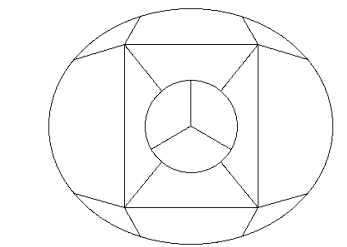
\includegraphics[width=0.5\columnwidth]{figs/fig1.png}
    \caption{}
    \label{fig:placeholder}
\end{figure} 
\begin{multicols}{4}
\begin{enumerate}
    \item 4
    \item 3
    \item 5
    \item 6
\end{enumerate}
\end{multicols}

\hfill (GATE PI 2024)

\item How many 4-digit positive integers divisible by 3 can be formed using only the digits $\cbrak{1, 3, 4, 6, 7}$, such that no digit appears more than once in a number?

\begin{multicols}{4}
\begin{enumerate}
    \item 24
    \item 48
    \item 72
    \item 12
\end{enumerate}
\end{multicols}

\hfill (GATE PI 2024)

\item The sum of the following infinite series is
\begin{align*}
2 + \frac{1}{2} + \frac{1}{3} + \frac{1}{4} + \frac{1}{8} + \frac{1}{9} + \frac{1}{16} + \frac{1}{27} + \cdots
\end{align*}

\begin{multicols}{4}
\begin{enumerate}
    \item $\frac{11}{3}$
    \item $\frac{7}{2}$
    \item $\frac{13}{4}$
    \item $\frac{9}{2}$
\end{enumerate}
\end{multicols}

\hfill (GATE PI 2024)

\item In an election, the share of valid votes received by the four candidates A, B, C, and D is represented by the pie chart shown. The total number of votes cast in the election were 1,15,000, out of which 5,000 were invalid.
Based on the data provided, the total number of valid votes received by the candidates B and C is \\

\begin{center}
\textbf{Share of valid votes}
\end{center}
\begin{figure}[H]
\centering
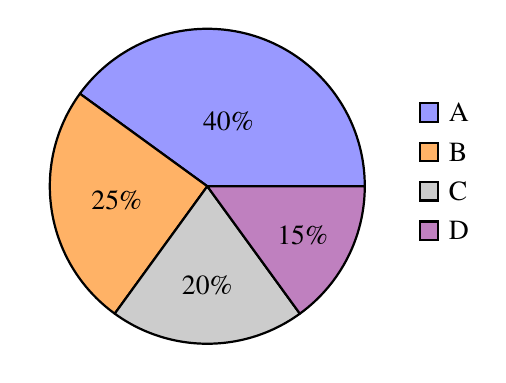
\begin{tikzpicture}
\pie[
text=legend,
radius=2,
color={blue!40!white, orange!60!white, gray!40!white, violet!50!white}
]{40/A, 25/B, 20/C, 15/D}
\end{tikzpicture}
\caption{Pie}
\end{figure}

\begin{multicols}{4}
\begin{enumerate}
    \item 45,000
    \item 49,500
    \item 51,750
    \item 54,000
\end{enumerate}
\end{multicols}

\hfill (GATE PI 2024)

\item Thousands of years ago, some people began dairy farming. This coincided with a number of mutations in a particular gene that resulted in these people developing the ability to digest dairy milk.
Based on the given passage, which of the following can be inferred?

\begin{enumerate}
    \item All human beings can digest dairy milk.
    \item No human being can digest dairy milk.
    \item Digestion of dairy milk is essential for human beings.
    \item In human beings, digestion of dairy milk resulted from a mutated gene.
\end{enumerate}

\hfill (GATE PI 2024)

\item The probability of a boy or a girl being born is 1/2. For a family having only three children, what is the probability of having two girls and one boy?

\begin{multicols}{4}
\begin{enumerate}
    \item $\frac{3}{8}$
    \item $\frac{1}{8}$
    \item $\frac{1}{4}$
    \item $\frac{1}{2}$
\end{enumerate}
\end{multicols}

\hfill (GATE PI 2024)

\item Person 1 and Person 2 invest in three mutual funds A, B, and C. The amounts they invest in each of these mutual funds are given in the table.

\begin{center}
\begin{tabular}{ll}
    \textbf{Group I} & \textbf{Group II} \\
    P. Ferrite & 1. Hexagonal Close Packed (HCP) \\
    Q. Austenite & 2. Body Centered Cubic (BCC) \\
    R. Martensite & 3. Body Centered Tetragonal (BCT) \\
    & 4. Face Centered Cubic (FCC)
\end{tabular}
\end{center}       

At the end of one year, the total amount that Person 1 gets is \rupee500 more than Person 2. The annual rate of return for the mutual funds B and C is 15\% each. What is the annual rate of return for the mutual fund A?

\begin{multicols}{4}
\begin{enumerate}
    \item 7.5\%
    \item 10\%
    \item 15\%
    \item 20\%
\end{enumerate}
\end{multicols}

\hfill (GATE PI 2024)

\item Three different views of a dice are shown in the figure below.

\begin{figure}[H]
\centering
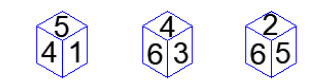
\includegraphics[width=0.5\columnwidth]{fig2.png}
\caption{}
\end{figure}

The piece of paper that can be folded to make this dice is

\begin{figure}[H]
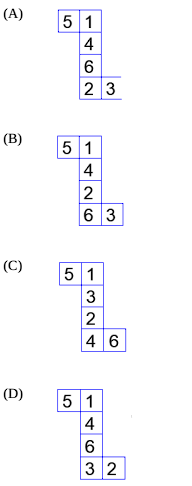
\includegraphics[width=0.3\columnwidth]{fig3.png}
\caption{}
\end{figure}


\hfill (GATE PI 2024)

\item Visualize two identical right circular cones such that one is inverted over the other and they share a common circular base. If a cutting plane passes through the vertices of the assembled cones, what shape does the outer boundary of the resulting cross-section make?

\begin{enumerate}
\begin{multicols}{2}
    \item A rhombus
    \item A triangle
    \item An ellipse
    \item A hexagon
\end{multicols}
\end{enumerate}

\hfill (GATE PI 2024)

\item In the Taylor series expansion of $\sin z$ around $z = 0$, the coefficient of the term $z^3$ is

\begin{multicols}{4}
\begin{enumerate}
    \item 0
    \item $\frac{1}{3}$
    \item $-\frac{1}{6}$
    \item $-\frac{1}{3}$
\end{enumerate}
\end{multicols}

\hfill (GATE PI 2024)

\item A vector field is given as $\mathbf{F}\brak{x,y} = \brak{100x + 100y},\mathbf{i} + \brak{-50x + 200y},\mathbf{j}$, where $\mathbf{i}$ and $\mathbf{j}$ are the unit vectors along the $x$ and $y$ axes in the Cartesian frame, respectively. Then the value of
\begin{align*}
\oint_c\ \textbf{F}\brak{x,y}.\textbf{dl}
\end{align*}
where $d\mathbf{l} = dx,\mathbf{i} + dy,\mathbf{j}$ is an elemental path taken over an anticlockwise circular contour $C$ of radius $r = 2$ is

\begin{figure}[H]
\centering
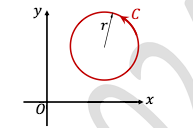
\includegraphics[width=0.5\columnwidth]{fig4.png}
\caption{}
\end{figure}

\begin{multicols}{4}
\begin{enumerate}
    \item $-100\pi$
    \item $-800\pi$
    \item $-400\pi$
    \item $400\pi$
\end{enumerate}
\end{multicols}

\hfill (GATE PI 2024)

\item A uniform cantilever beam of length $L$ and flexural rigidity $EI$ is loaded by a force $F$ as shown in the figure. Assuming that the Euler-Bernoulli beam theory is applicable here, the magnitude of the static deflection at the free end of the beam is

\begin{figure}[H]
\centering
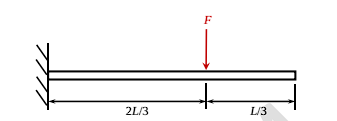
\includegraphics[width=0.5\columnwidth]{fig5.png}
\caption{}
\end{figure}

\begin{multicols}{4}
\begin{enumerate}
    \item $\frac{FL^3}{6EI}$
    \item $ \frac{14FL^3}{81EI}$
    \item $\frac{5FL^3}{27EI}$
    \item $ \frac{7FL^3}{48EI}$
\end{enumerate}
\end{multicols}

\hfill (GATE PI 2024)

\item A thin copper wire carries electric current and is insulated by putting a sleeve, of thickness $t$, over it. In steady state conditions, the rate of heat loss from the insulated wire per unit length is $Q$. Which of the following is TRUE?

\begin{enumerate}
    \item $Q$ increases monotonically with $t$.
    \item $Q$ decreases monotonically with $t$.
    \item $Q$ first increases with increase in $t$, and then it decreases with further increase in $t$.
    \item $Q$ first decreases with increase in $t$, and then it increases with further increase in $t$.
\end{enumerate}

\hfill (GATE PI 2024)

\item The solidification time of a cube and a cylinder of the same material, produced through the same sand casting process, is found to be equal. Each side of the cube is $a$, and the radius and the length of the cylinder are $r$ and $4r$, respectively. If the solidification time is governed by Chvorinov's equation, then the ratio $r/a$ is

\begin{multicols}{4}
\begin{enumerate}
    \item $\frac{1}{3}$
    \item $\frac{5}{12}$
    \item $\frac{7}{12}$
    \item $\frac{5}{9}$
\end{enumerate}
\end{multicols}

\hfill (GATE PI 2024)

\item Match each of the listed defects in deep drawing cup with the corresponding reason in the table.\newline

\begin{tabular}{|c|c|c|}
     \hline
     \textbf{Mineral} & \textbf{Modal abundance \brak{\%}} & \textbf{Partition coefficient}\\
     \hline
     Clinopyroxene & $45$ & $0.506$ \\
      \hline
      Orthopyroxene & $40$ & $0.42$ \\
      \hline
      Olivine & $10$ & $0.045$ \\
      \hline
      Plagioclase & $05$ & $0.019$ \\
      \hline
\end{tabular}

\begin{enumerate}
\begin{multicols}{2}
\item  P-3, Q-4, R-2, S-1 
\item  P-4, Q-1, R-3, S-2 
\item P-3, Q-1, R-2, S-4 
\item P-2, Q-3, R-1, S-4
\end{multicols}
\end{enumerate}

\hfill (GATE PI 2024)

\item Which one of the following pure metals has the hexagonal close packed (HCP) crystal structure at room temperature?
\begin{enumerate}
    \item Magnesium
    \item Iron
    \item Aluminium
    \item Copper
\end{enumerate}

\hfill (GATE PI 2024)

\item To create 12 divisions on a disc by using simple indexing and dividing head on a horizontal milling machine, choose the correct option for the rotation of the crank pin.

\begin{enumerate}
    \item 3 full rotations and 5 holes on a 15-hole circle
    \item 5 full rotations and 4 holes on a 16-hole circle
    \item 3 full rotations and 5 holes on a 18-hole circle
    \item 5 full rotations and 4 holes on a 20-hole circle
\end{enumerate}

\hfill (GATE PI 2024)

\item The following layout of four departments P, Q, R and S is provided as input to CRAFT (Computerized Relative Allocation of Facilities Technique). Which one of the following department pairs cannot be considered

\begin{figure}[H]
\centering
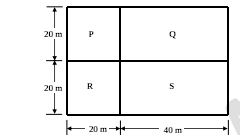
\includegraphics[width=0.5\columnwidth]{fig6.png}
\caption{}
\end{figure}


\begin{enumerate}
\begin{multicols}{4}
    \item P and Q
    \item R and S
    \item P and R
    \item Q and R
    \end{multicols}
\end{enumerate}

\hfill (GATE PI 2024)

\item Which of the following concepts is not closely inter-related with INTERCHANGEABILITY in the context of product design?

\begin{enumerate}
\begin{multicols}{4}
    \item Standardization
    \item Simplification
    \item Diversification
    \item Specialization
\end{multicols}
\end{enumerate}

\hfill (GATE PI 2024)

\item Which one of the following THERBLIGS does not advance the progress of the work and can be eliminated by applying the principles of motion economy?

\begin{enumerate}
\begin{multicols}{2}
    \item Move
    \item Grasp
    \item Search
    \item Preposition
    \end{multicols}
\end{enumerate}

\hfill (GATE PI 2024)

\item If work sampling is carried out using a large number of observations, then the required sample size is estimated using

\begin{multicols}{2}
\begin{enumerate}
    \item Poisson distribution
    \item Uniform distribution
    \item Normal distribution
    \item Exponential distribution
\end{enumerate}
\end{multicols}

\hfill (GATE PI 2024)

\item Which of the following is NOT an assumption of a linear programming problem?

\begin{enumerate}
\begin{multicols}{2}
    \item Proportionality
    \item Additivity
    \item Integrality
    \item Certainty
\end{multicols}
\end{enumerate}

\hfill (GATE PI 2024)

\item In a single server Markovian queuing system, if the customers arrive following the Poisson distribution, then the inter-arrival time follows

\begin{multicols}{2}
\begin{enumerate}
    \item Poisson distribution
    \item Uniform distribution
    \item Exponential distribution
    \item Binomial distribution
\end{enumerate}
\end{multicols}

\hfill (GATE PI 2024)

\item Which one of the following methods requires the least amount of data for forecasting?

\begin{enumerate}
    \item Econometric forecasting method
    \item Linear regression method
    \item ARIMA method
    \item Simple exponential smoothing method
\end{enumerate}

\hfill (GATE PI 2024)

\item Which one of the following is not true about Total Productive Maintenance (TPM)?

\begin{enumerate}
    \item It allows operators to perform preventive maintenance on the machines.
    \item It allows operators to perform reactive maintenance on the machines.
    \item It is consistent with the Just-in-Time (JIT) system.
    \item It is consistent with the Lean system.
\end{enumerate}

\hfill (GATE PI 2024)

\item In a complex function, $f\brak{x,y} = u\brak{x,y} + i v\brak{x,y}$, $i$ is the imaginary unit, and $x, y, u\brak{x,y}$, and $v\brak{x,y}$ are real. If $f\brak{x,y}$ is analytic, then which of the following equations is/are TRUE?
\begin{enumerate}
\setlength{\itemsep}{1em}
\item $\frac{\partial^2 u}{\partial x^2} + \frac{\partial^2 u}{\partial y^2} = 0$
\item $\frac{\partial^2 v}{\partial x^2} + \frac{\partial^2 v}{\partial y^2} = 0$
\item $\frac{\partial^2 u}{\partial x^2} + \frac{\partial^2 v}{\partial y^2} = 0$
\item $\left( \frac{\partial u}{\partial x} \right) \left( \frac{\partial v}{\partial x} \right) + \left( \frac{\partial u}{\partial y} \right) \left( \frac{\partial v}{\partial y} \right) = 0$
\end{enumerate}

\hfill (GATE PI 2024)

\item For a mild steel specimen subjected to uniaxial tensile load, which of the following is/are TRUE?
\begin{enumerate}
    \item The engineering stress-strain curve is linear within the elastic limit.
    \item The specimen fails in cup and cone type fracture.
    \item The true stress is always more than the engineering stress at any finite strain.
    \item The specimen does not regain its original dimensions after complete unloading from an initial stress above the yield stress.
\end{enumerate}

\hfill (GATE PI 2024)

\item Which among the following is/are TRUE for friction stir welding (FSW) process?


\begin{enumerate}
    \item It can be used to produce lap, butt and tee joints.
    \item A non-consumable rotating tool with shoulder and pin is used to melt the work-piece material.
    \item Retreating side of the weld is where the linear velocity vector at a point on that side of the rotating tool and the welding direction are opposite.
    \item Advancing side of the weld is where the linear velocity vector at a point on that side of the rotating tool and the welding direction are opposite.
\end{enumerate}

\hfill (GATE PI 2024)

\item Which of the following areas is/are supply chain decision(s)?

\begin{enumerate}
\begin{multicols}{2}
    \item Location
    \item Inventory
    \item Distribution
    \item Machine scheduling
    \end{multicols}
\end{enumerate}

\hfill (GATE PI 2024)

\item If $X$ is a continuous random variable with the probability density function
\begin{align*}
f(x) = 
\begin{cases}
\frac{K}{4}, & 0 \leq x \leq 1 \\
0, & \text{otherwise}
\end{cases}
\end{align*}
then the value of $K$ is \dots (Answer in integer)

\hfill (GATE PI 2024)

\item If
\begin{align*}
\lim_{x \to 1} \brak{ \frac{x^2 - 2ax + b}{x-1} } = 8 
\end{align*}
then $\brak{a-b}$ is \dots (Answer in integer)

\hfill (GATE PI 2024)

\item In the truss shown in the figure, member AC is an inextensible string, other members are rigid, and ABCD is a square with each side of length $a$. The maximum value of force $F$ (in kN) for which the truss will remain in static equilibrium is \dots . (Rounded off to 2 decimal places)

\begin{figure}[H]
\centering
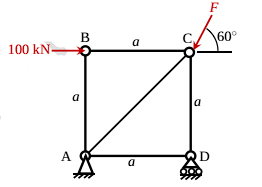
\includegraphics[width=0.5\columnwidth]{fig7.png}
\caption{}
\end{figure}

\hfill (GATE PI 2024)

\item An offset slider-crank mechanism is shown in the figure. If the length $l=10$ cm, then the stroke length (in cm) of the slider is \dots . (Rounded off to 1 decimal place)

\begin{figure}[H]
\centering
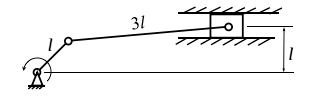
\includegraphics[width=0.5\columnwidth]{fig8.png}
\caption{}
\end{figure}

\hfill (GATE PI 2024)

\item A blank of 100 mm diameter is to be cut out of a 2 mm thick sheet through blanking operation. If the radial clearance between the punch and die is 6\% of the sheet thickness then the diameter (in mm) of the punch is \dots . (Rounded off to 2 decimal places)

\hfill (GATE PI 2024)

\item If A =
$
\myvec{
a & b \\
c & -a 
} 
$
is a matrix such that $A^2=I$, where $I$ is an identity matrix, then which of the following is TRUE?

\begin{enumerate}
    \item 1 $+$ $a^2$ $+$ $bc$ $=$ 0
    \item 1 $-$ $a^2$ $+$ $bc$ $=$ 0
    \item 1 $-$ $a^2$ $-$ $bc$ $=$ 0
    \item 1 $+$ $a^2$ $-$ $bc$ $=$ 0
\end{enumerate}

\hfill (GATE PI 2024)

\item In the iron-carbon equilibrium phase diagram, the temperature and composition of the eutectoid point are 727 $^\circ$C and 0.77 weight\% carbon, respectively. If a steel specimen with 1.2 weight\% carbon is cooled from 1000 $^\circ$C to the room temperature, then the fraction of pro-eutectoid cementite phase in the steel is \dots (Rounded off to 2 decimal places)

\begin{multicols}{4}
\begin{enumerate}
    \item 0.07
    \item 0.93
    \item 0.18
    \item 0.12
\end{enumerate}
\end{multicols}

\hfill (GATE PI 2024)

\item For polymers, match each process with the most suitable a

\begin{table}[htbp]
  \centering
  \caption{Table-3}
  \label{table3}
  \begin{tabular}{cc}
  \textbf{Processing Technique} & \textbf{Producct} \\ \\
    P. Calendering & 1. Pipes \\
    Q. Extrusion & 2. Disposable cups \\
    R. Injection moulding & 3. Sheets \\
    S. Thermoforming & 4. Nylon gears \\
  \end{tabular}
\end{table}

\begin{enumerate}
\item P-3, Q-1, R-2, S-4
\item P-2, Q-3, R-4, S-1
\item P-4, Q-2, R-1, S-3
\item P-3, Q-1, R-4, S-2
\end{enumerate}

\hfill (GATE PI 2024)

\item In a forming operation, the plastic deformation of a steel specimen starts under plane stress condition, where the principal stresses are $\sigma_1=200$ Mpa and $\sigma_2=100$ Mpa. If the steel specimen follows von-Mises yield criterion, then the uniaxial tensile yield strength (in Mpa) of this steel material is \dots (Rounded off to 1 decimal place)

\begin{multicols}{4}
\begin{enumerate}
\item 173.2
\item 200.0
\item 100.0
\item 223.6
\end{enumerate}
\end{multicols}

\hfill (GATE PI 2024)

\item Match the configurations of the listed 3 degrees-of-freedom industrial robots with the type of joints.

\begin{center}
\begin{tabular}{|c|c|c|}
    \hline
    Task & Task time (Seconds) & Immediate predecessor(s) \\
    \hline
    P & 20 & - \\ \hline
    Q & 25 & P \\  \hline
    R & 10 & Q \\ \hline
    S & 15 & Q \\ \hline 
    T & 25 & R, S \\    \hline
\end{tabular}
\end{center}

\begin{enumerate}
\item P-3, Q-1, R-2, S-4
\item P-4, Q-3, R-1, S-2
\item P-4, Q-2, R-1, S-3
\item P-3, Q-1, R-4, S-2
\end{enumerate}


\hfill (GATE PI 2024)

\item A project has six activities and the precedence relationship among them is shown in the table.

\begin{table}[h!]
\centering
\begin{tabular}{|c|c|c|c|}
\hline
\textbf{Pressure} & \textbf{Temperature} & \multicolumn{2}{c|}{\textbf{Specific enthalpy}} \\ \cline{3-4} 
\textbf{(kPa)} & \textbf{($^\circ$C)} & $h_f$ (kJ/kg) & $h_g$ (kJ/kg) \\ \hline
150.9 & $-20$ & 17.82 & 178.74 \\ \hline
500 & 15.6 & 50.64 & 195.01 \\ \hline
\end{tabular}
\end{table}
 The minimum number of dummy activities needed to draw an activity-on-arrow (AOA) representation of the project network is \dots

\begin{enumerate}
\begin{multicols}{4}
\item 0
\item 1
\item 2
\item 3
\end{multicols}
\end{enumerate}

\hfill (GATE PI 2024)

\item  Consider the following linear programming problem with two decision variables $x_1$ and $x_2$. There are three constraints involving resources R1, R2 and R3 as indicated.

Maximize
\begin{align*}
    Z = 6x_1 + 5x_2
\end{align*}

Subject to
\begin{align*}
2x_1 + 5x_2 \leq 40 \quad \text{R1} \\
2x_1 + x_2 \leq 22 \quad \text{R2} \\
x_1 + x_2 \leq 13 \quad \text{R3} \\
x_1 \geq 0,\quad x_2 \geq 0 
\end{align*}

The optimal solution of the problem is: $x_1 = 9$ and $x_2 = 4$.

For which one of the following options, the shadow price of the resource(s) will have non-zero value(s)?

\begin{multicols}{2}
\begin{enumerate}
\item R1, R2 and R3
\item R1 and R2
\item R2 and R3
\item R1 only
\end{enumerate}
\end{multicols}

\hfill (GATE PI 2024)

\item Choose the item(s) which is/are required to make an eccentric hole on a disc, as shown, using a lathe.

\begin{figure}[H]
\centering
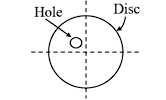
\includegraphics[width=0.5\columnwidth]{fig9.png}
\caption{}
\end{figure}

\begin{multicols}{2}
\begin{enumerate}
\item Single point cutting tool
\item Four jaw chuck
\item Drill bit
\item Three jaw chuck
\end{enumerate}
\end{multicols}

\hfill (GATE PI 2024)

\item Which of the following statement(s) is/are TRUE for a given acceptance sampling plan?

\begin{enumerate}
\item Type II error decreases with an increase in type I error.
\item The probability of rejecting a good quality lot is producer's risk.
\item Type II error decreases with a decrease in sample size.
\item The probability of rejecting a good quality lot is consumer's risk.
\end{enumerate}

\hfill (GATE PI 2024)

\item Seven cards numbered 1 to 7 are placed in a box. After thoroughly mixing all the cards, one card is drawn at random.

If it is known that the number on the card drawn is odd, then the probability that the number on the card drawn is greater than 4 is \dots.

(Answer in integer)

\hfill (GATE PI 2024)

\item The following differential equation governs the evolution of variable $x(t)$ with time $t$, $t \geq 0$.

\begin{align*}
\frac{d^2x}{dt^2} + 4x = e^{-t}
\end{align*}

Given the initial conditions $x = 0$ and $\frac{dx}{dt} = 0$ at $t = 0$, the value of $x$ at $t = \pi/8$ is \dots .
(Rounded off to 3 decimal places)

\hfill (GATE PI 2024)

\item The values of function $y\brak{x}$ at discrete values of $x$ are given in the table. The value of $\int_0^4 y\brak{x}dx$, using Trapezoidal rule is \dots .
(Rounded off to 1 decimal place)

\begin{table}[htbp]
  \centering
  \caption{Table-6}
  \label{tab:tables/table6.tex}
  \begin{tabular}{cc}
  \textbf{Reagent} & \textbf{Function} \\ \\
    P.Ammonia  & 1. Prevent storage hardening \\
    Q. Hydroxylamine & 2. Delay plugging mechanism \\
    R. Formic acid & 3. Stabilizer \\
    S. Ethephone & 4. Coagulating agent \\
  \end{tabular}
\end{table}

\hfill (GATE PI 2024)

\item An irrigation pump is used to draw water from a pond. One end of a 5.05 cm diameter hose pipe is connected to the outlet of the pump at 1.02 m below the surface level, and just after the pump, the static gauge pressure and flow rate of the water are 50 kPa and 8 kg/s, respectively. The pumped water is discharged at the ground level through a nozzle. Assume that the flow through the hose pipe and nozzle is steady and laminar, and frictional and viscous losses are negligible. The density of water is 1000 kg/m$^3$ and the acceleration due to gravity is 9.81 m/s$^2$. If the static pressure at the nose/exit of the nozzle just reduces to atmospheric pressure then the nose diameter (in cm) of the nozzle is \dots . (Rounded off to 2 decimal places)

\hfill (GATE PI 2024)

\item In an air-standard Otto cycle, the pressure and temperature of air just before the compression stroke are 200 kPa and 26.85$^\circ$C, respectively. The combustion process is assumed to be a constant volume process, where 1.02 MJ/kg heat is added. The cycle efficiency is 50\%. The adiabatic index $\gamma$ and specific heat at constant volume $c_v$ can be considered to be constant during the process (corresponding values taken at the mean cycle temperature).

Assuming that the ideal gas law is applicable, $\gamma = 4/3$ and $c_v = 0.85$ kJ/kg-K, the maximum pressure (in MPa) reached during the cycle is \dots . (Rounded off to 1 decimal place)

\hfill (GATE PI 2024)

\item A metallic cylindrical pressure vessel, used to store compressed air in a plant, has 1 mm mean radius and 4 mm wall thickness. The maximum allowable normal and shear stresses in the cylindrical portion of the vessel are 100 MPa and 40 MPa, respectively. Considering only these data in the design, the maximum allowable internal gauge pressure (in MPa) of the compressed air is \dots . (Rounded off to 2 decimal places)

\hfill (GATE PI 2024)

\item A flat belt drive with pulley of $r = 20$ cm radius is designed to transmit 6.283 kW power at 600 RPM. In the figure, $\tau$ is the corresponding torque. If the coefficient of static friction between the belt and the pulley is $0.3$, then the minimum value of the tightening force $F$ (in kN) required to prevent the belt slip is \dots . (Rounded off to 2 decimal places)

\begin{figure}[H]
\centering
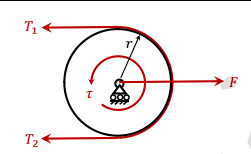
\includegraphics[width=0.5\columnwidth]{fig10.png}
\caption{}
\end{figure}

\hfill (GATE PI 2024)

\item Mild steel plates are welded to make butt joints by arc welding with 85\% heat transfer efficiency ignoring other losses. The first weld joint is made by selecting arc voltage of 30V and current of 180A with a welding speed of 6mm/s. Using identical plates, a second weld joint is made with the same arc voltage and a welding speed of 8mm/s. If both the welds have the same heat input, then the welding current (in A) for the second weld joint is \dots . (Answer in integer)

\hfill (GATE PI 2024)

\item In a single pass cold rolling operation, a flat plate is reduced to a thickness of 3mm. In this operation, two rolls of diameter 400mm each are rotating in opposite direction at 300RPM, and the elastic deflection of these rolls is negligible. The angle of bite is $10^\circ$. If the neutral point is present at an angle of $7^\circ$ from the exit side, then the thickness of the plate (in mm) at the neutral point is \dots . (Rounded off to 1 decimal place)

\hfill (GATE PI 2024)

\item In a sand mold, a sprue of height $h_2 = 200$ mm is to be provided for maintaining the molten metal flow rate of $10^6$ mm$^3$/s. The height of liquid column above the point 2 is kept constant at $h_c = 25$ mm. The cross-sectional areas of the sprue at points 2 and 3 are $A_2$ and $A_3$, respectively. The points 1 and 3 are at the atmospheric pressure. Assuming the gauge pressure at point 2 to be zero as the limiting case to prevent aspiration effect, the ratio $A_3/A_2$ is \dots . (Rounded off to 2 decimal places)

\begin{figure}[H]
\centering
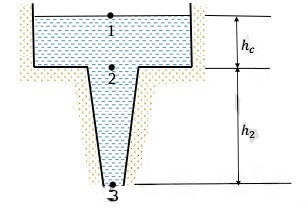
\includegraphics[width=0.5\columnwidth]{fig11.png}
\caption{}
\end{figure}

\hfill (GATE PI 2024)

\item The following data are given in relation to turning operation of a cylindrical workpiece.

Diameter of the workpiece = 160 mm, length of the workpiece = 190 mm, cutting velocity = $80\pi$ m/min, and tool feed = 0.2 mm/rev.

Assuming the approach and the overrun of the tool to be 5 mm each, the machining time (in minutes) is \dots . (Answer in integer)

\hfill (GATE PI 2024)

\item A CNC milling operation is carried out by moving the tool from the point A to point B in anti-clockwise direction to cut a slot of quarter circle with center at C, as shown. The coordinates of the points A and B are (0,0) and (10,10), respectively. All dimensions are in mm. If the feed rate at point P along x-axis is 6 mm/min, then the feed rate (in mm/min) at point P along y-axis is \dots . (Rounded off to 1 decimal place)

\begin{figure}[H]
\centering
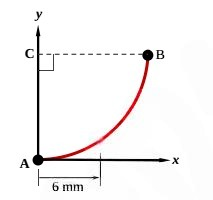
\includegraphics[width=0.5\columnwidth]{fig12.png}
\caption{}
\end{figure}
\hfill (GATE PI 2024)

\item The pitch of a metric screw thread is calculated from pitch circle diameter measurement through two-wire method. If the thread is single-start with calculated pitch of 1.4 mm then the diameter (in mm) of the best-wire is \dots . (Rounded off to 2 decimal places)

\hfill (GATE PI 2024)

\item During orthogonal turning, the cutting speed, feed and depth of cut are set as 2 m/s, 0.2 mm/rev and 2 mm, respectively. The specific cutting energy (neglecting the effect of feed force on the total cutting power) is 2 J/mm$^3$. The main cutting force (in N) is \dots . (Answer in integer)

\hfill (GATE PI 2024)
\item Electro-chemical machining is performed on a flat copper workpiece. If the material removal rate is $2$ cm$^3$/min throughout the process, then the required current (in A) is \dots . (Rounded off to 1 decimal place)

Copper properties: Melting point = 1085 $^\circ$C, density = 9 g/cm$^3$, gram atomic weight = 63, and valency of dissolution = 2

Faraday's constant = 96500 C

Stefan-Boltzmann constant $= 5.67 \times 10^{-8}$ W/m$^2$-K$^4$

\hfill (GATE PI 2024)

\item A repairable machine operated for 2400 hours in a year and for that year the machine broke down 8 times. The mean time to repair including waiting time is found to be 20 hours for that year.

If the mean time to repair including waiting time could have been reduced to 10 hours for that year, then the improvement in the availability of that machine would be \dots (Rounded off to 2 decimal places)

\hfill (GATE PI 2024)

\item In a time study, the average time taken for packaging a product in a warehouse by a worker with 120\% performance rating is observed as 9 minutes. Assuming an allowance of 10\% of the standard time, the standard time (in minutes) for packaging is \dots (Answer in integer)

\hfill (GATE PI 2024)

\item An assembly line consists of three work stations (S1, S2 and S3) in series to assemble a toy. The times required to perform tasks at these stations are 6, 4 and T minutes, respectively. If the efficiency of the assembly line in the steady state is 75\%, then the maximum value of T (in minutes) is \dots (Answer in integer)

\hfill (GATE PI 2024)


\item A company purchased two machines, Machine A and Machine B, at the same time. The purchase price, estimated useful life and the estimated salvage value of the two machines are given in the table.

\begin{table}[htbp]
  \centering
  \caption{Table-7}
  \label{tab:tables/table7.tex}
  \begin{tabular}{cc}
\textbf{Additives} & \textbf{Fuction}\\

P. Molybdenum disulphide & 1. Heat stabilizer \\
Q. Glycerol monostearate & 2. UV-absorber \\
R. Tribasic lead sulphate & 3. Antistatic agent \\
S. 2-hydroxybenzophenone & 4. Solid layer lubricant \\
  
  
  
  \end{tabular}
\end{table}

Using the straight-line depreciation method for both the machines, the difference (in INR) between the value of Machine A and the value of Machine B at the end of five years is \dots . (Answer in integer)

\hfill (GATE PI 2024)

\item A company orders an item using the classical economic order quantity formula. If the ordering cost per order is increased by 20\% and the demand per unit time is also increased by 20\%, then the time between orders increases (in \%) by \dots . (Answer in integer)

\hfill (GATE PI 2024)

\item Five jobs A, B, C, D and E are available at time t= 0 for processing at a machine, and their processing times are listed.

\begin{table}[htbp]
  \centering
  \caption{Table-8}
  \label{table8}
  \begin{tabular}{cc}
  \textbf{Group-I} & \textbf{Group-II} \\ \\
    P. Corn & 1. Lycopene \\
    Q. Red pepper & 2. $\beta$-Carotene \\
    R. Pumpkin & 3. Capsanthin \\
    S. Tomato & 4. Lutein \\
  \end{tabular}
\end{table}

If the jobs are processed using the shortest processing time (SPT) rule, the average flow time (in days) is \dots . (Rounded off to 1 decimal place)

\hfill (GATE PI 2024)













\end{enumerate}




\end{document}
